\documentclass[12pt]{article}

\usepackage{graphics}
\usepackage{epsfig}
\usepackage{times}
\usepackage{amsmath,amsfonts,amssymb}

\usepackage{subfig,float} % for sub figures

\usepackage{color, colortbl}

\definecolor{LightGray}{gray}{.9} % for table rows

\usepackage{multirow} % for the table 

\usepackage[nottoc]{tocbibind}

\usepackage{pgfgantt}

%\topmargin      0.0in
%\headheight     0.0in
%\headsep        0.0in
\oddsidemargin  0.0in
\evensidemargin 0.0in
%\textheight     9.0in
\textwidth      6.5in

\title{{\small University of New Mexico} \\ ~\\ 
Adaptive Mesh Based Surface Reconstruction For Noisy and Incremental Point Cloud Data Sets}

\author{ 
\small A thesis proposal submitted in partial fulfilment for the degree of Master’s of Science \\ ~\\
{Lucas Chavez}  \\
{\small lucasc@unm.edu} \\ ~\\
Department of Mechanical Engineering \\ 
University of New Mexico \\ ~\\
Advior \\ Dr. Ron Lumia \\ ~\\
December 2012
}

\date{}

\begin{document}
\pagestyle{plain}
\pagenumbering{roman}
\maketitle

\pagenumbering{arabic}

\section{Approach}
\label{ch:approach}

A clear idea of the algorithmic structure of the proposed system is
given by the System Flow Diagram in Figure \ref{fig:SD}. A basic
description of the main variables can be found in Table \ref{tab:var}.
The inputs to the system are RGB-D data from a Kinect-style sensor $D$
and the pose of the sensor $P$. The end goal of the system is to update
the current mesh representation in each iteration. This update is
represented by the last step in the System Flow Diagram. We can see that
the update step is primed by two distinct processes. In the diagram,
each processes is signified  by a blue background. On the left hand side
we have a processes which is named the Triangulation Process. This
process defines a triangulation $T$ based on the current depth image. On
the right hand side we have a processes which is named the
Categorization Process. This process categorizes the measurements based
on the effect they will have on the model. This triangulation
and categorization will be used by the update procedure to efficiently
evolve the map based on the current sensor measurements.                                                                 

\begin{figure}[h]
  \centering
    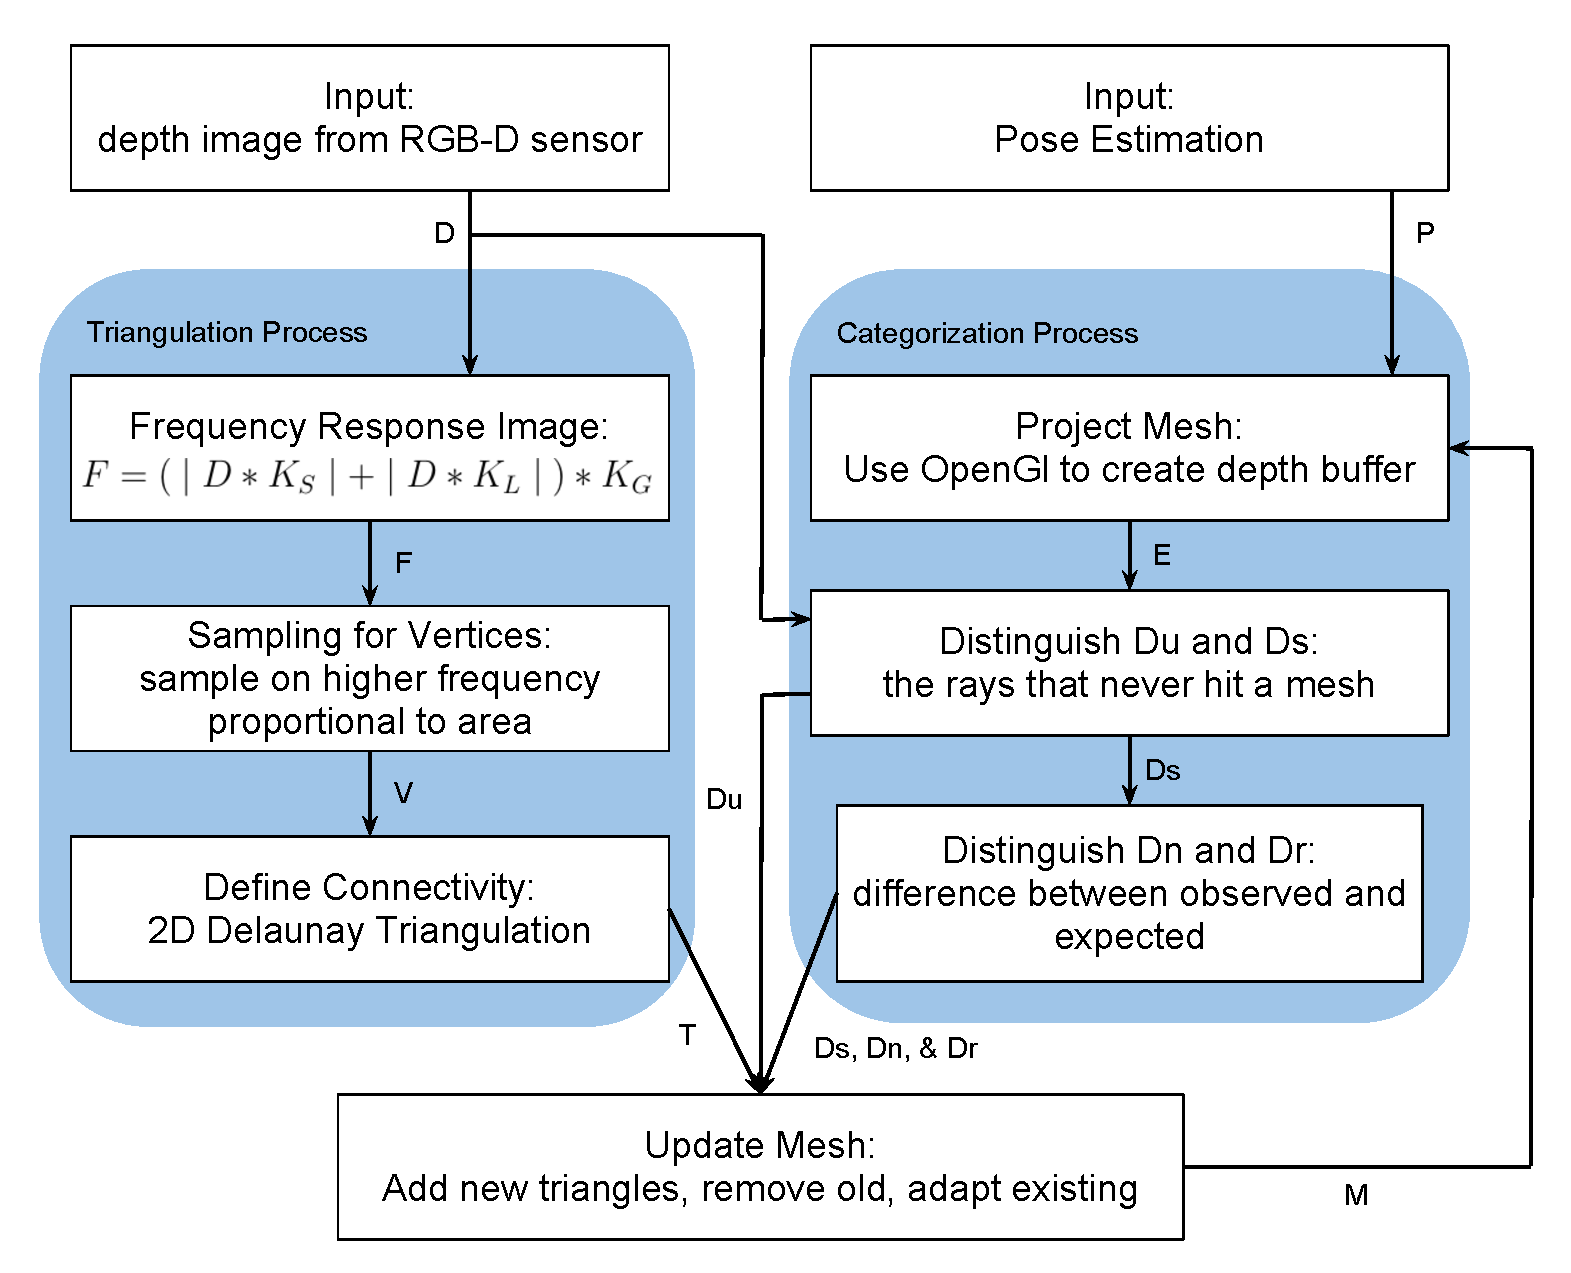
\includegraphics[height=0.8\textwidth]{SD.pdf}
  \caption{System Flow Diagram}
  \label{fig:SD}
\end{figure}

\begin{table}[h]
\begin{center}
\begin{tabular}{|c|l|}
\hline
{\bf Variable Name} & \multicolumn{1}{|c|}{{\bf Description}} \\
\hline
\rowcolor{LightGray} $D$ & Depth image from RGB-D sensor \\ 
$F$ & Frequency response image \\
\rowcolor{LightGray} $K_S,K_L,\text{ and }K_G$ & Image convolution operators \\
$V \text{ and } C$ & Mesh vertices and connectivity of the current triangulation \\
\rowcolor{LightGray} $T$ & Current triangulation. Contains both $V$ and $C$ \\
$P$ & The known pose of the sensor \\
\rowcolor{LightGray} $E$ & Expected depth image \\ 
$D_u,D_s,D_n,\text{ and } D_r$ & Regions of the $D$ classified by the
effect on the model \\ 
\hline
\end{tabular}
\end{center}
\caption{Basic description of the main variables}
\label{tab:var}
\end{table}

In the remaining sections of the Approach we will discuss the two
processes which prime the update step in detail. Finally, we will
discuss how the outputs are used to update the existing mesh map.

\subsection{Triangulation Process}

The goal of this process is to use the current depth image $D$ to estimate a
mesh of the current view of the of the environment. We can see a
simplified system flow chart of this process in Figure \ref{fig:SD_CT}.
Also, we can see an example of the outputs of the process using an
example input in Figure \ref{fig:O_CT}. It is important to
remember that not all of these new elements will be used in the update.
The decision of which elements from $T$ to use will be based on the
output of the Classification Process. 

\begin{figure}[h!]
  \centering
    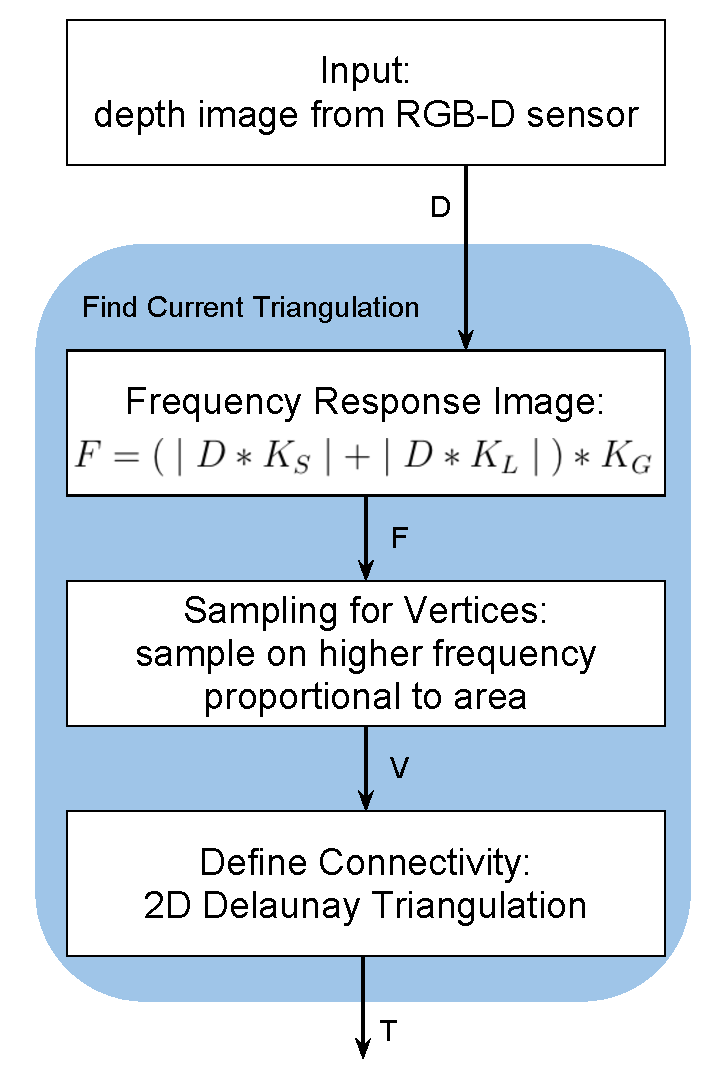
\includegraphics[height=0.5\textwidth]{SD_CT.pdf}
  \caption{Flow Diagram of Current Triangulation Process}
  \label{fig:SD_CT}
\end{figure}

\begin{figure}[h]
\centering
\subfloat[Color Image]{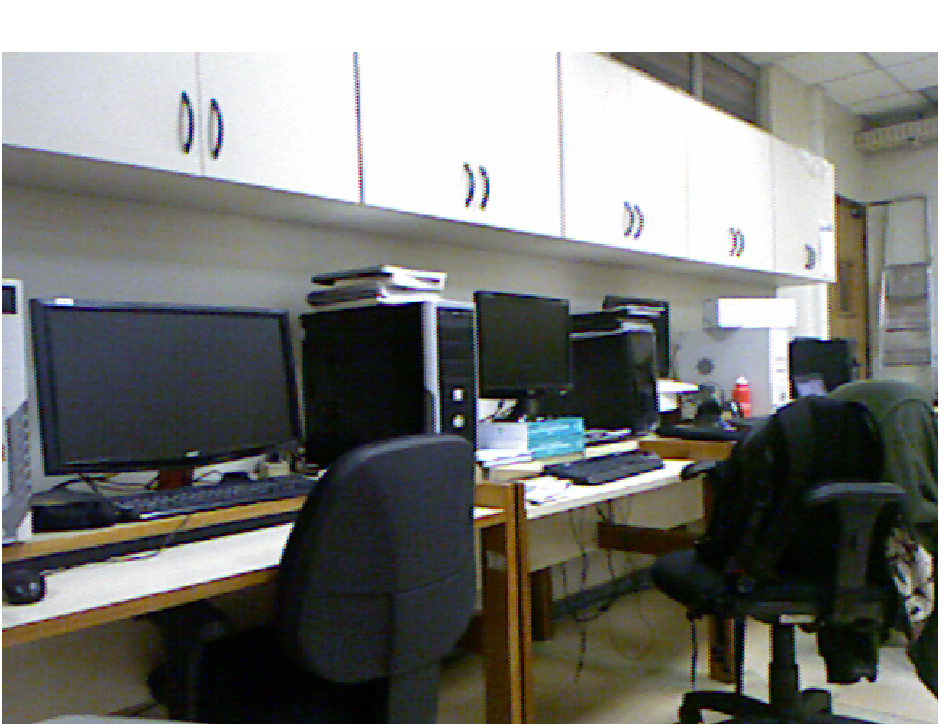
\includegraphics[width=.3\textwidth]{m_photo.pdf}} \quad
\subfloat[Depth Image $D$]{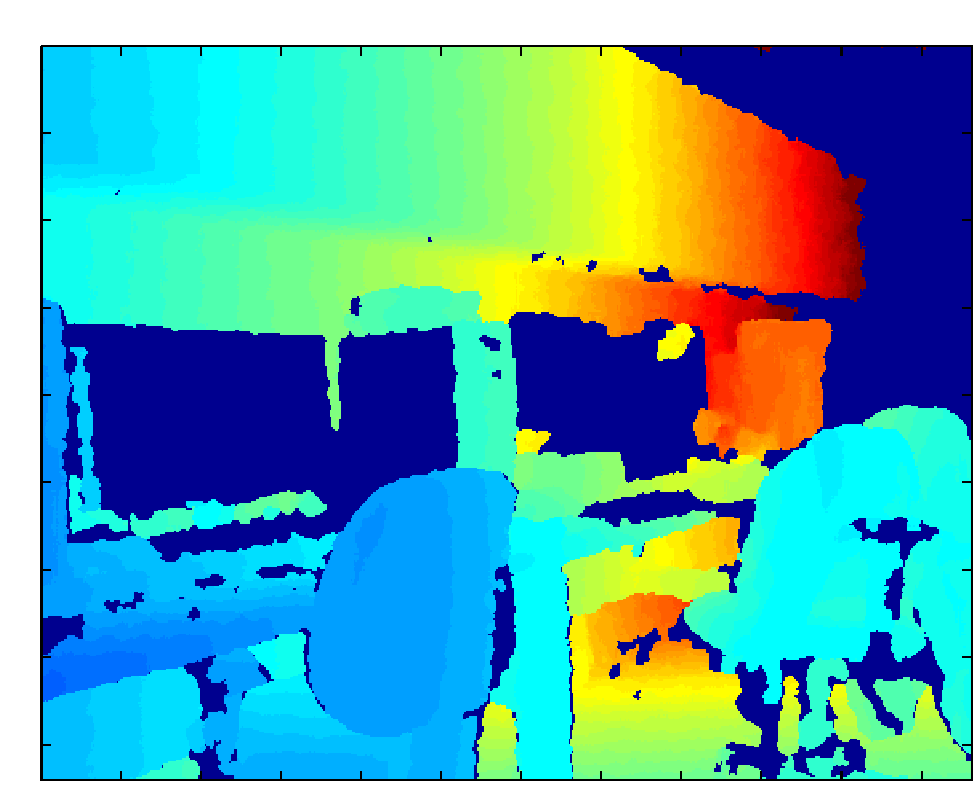
\includegraphics[width=.3\textwidth]{m_depth.pdf}} \quad
\subfloat[High Frequency Response $F$]{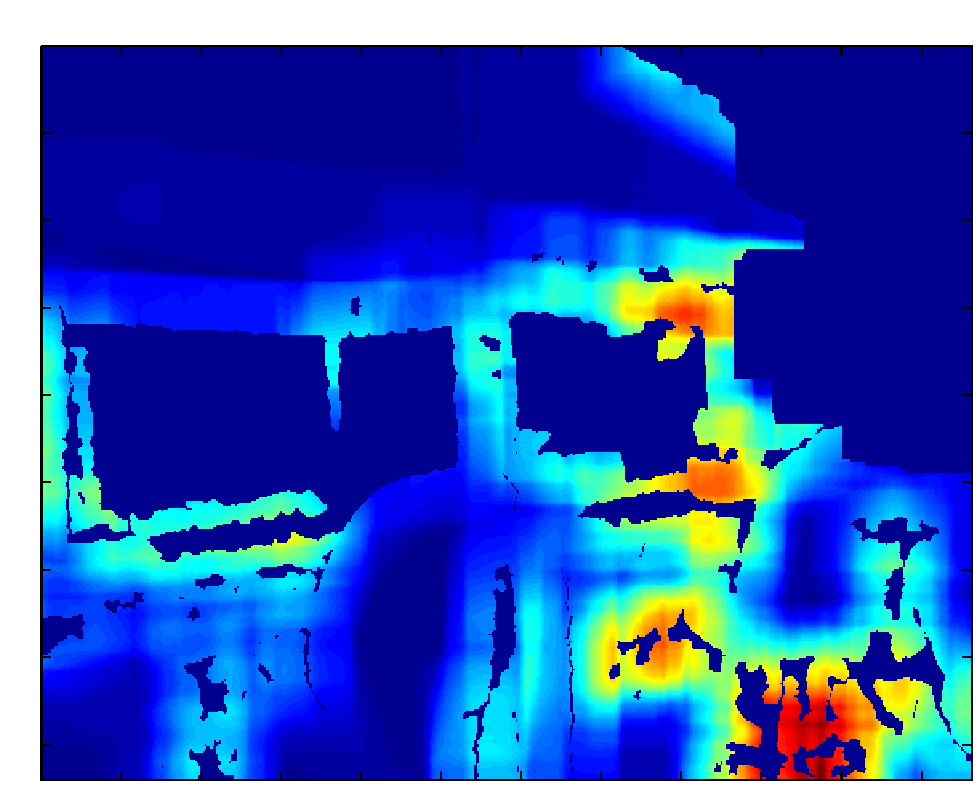
\includegraphics[width=.3\textwidth]{m_freqn.pdf}} \\
\subfloat[After Histogramming $F$]{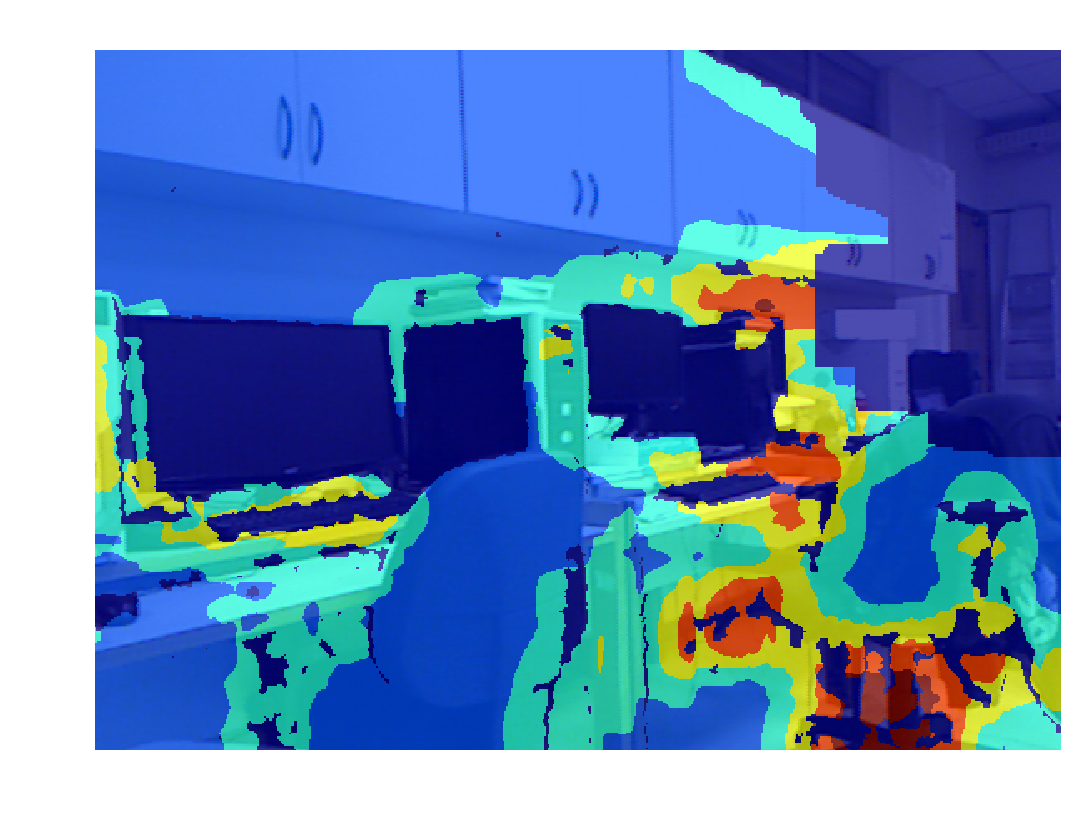
\includegraphics[width=.3\textwidth]{m_ihist.pdf}} \quad
\subfloat[Sampled Vertices $V$]{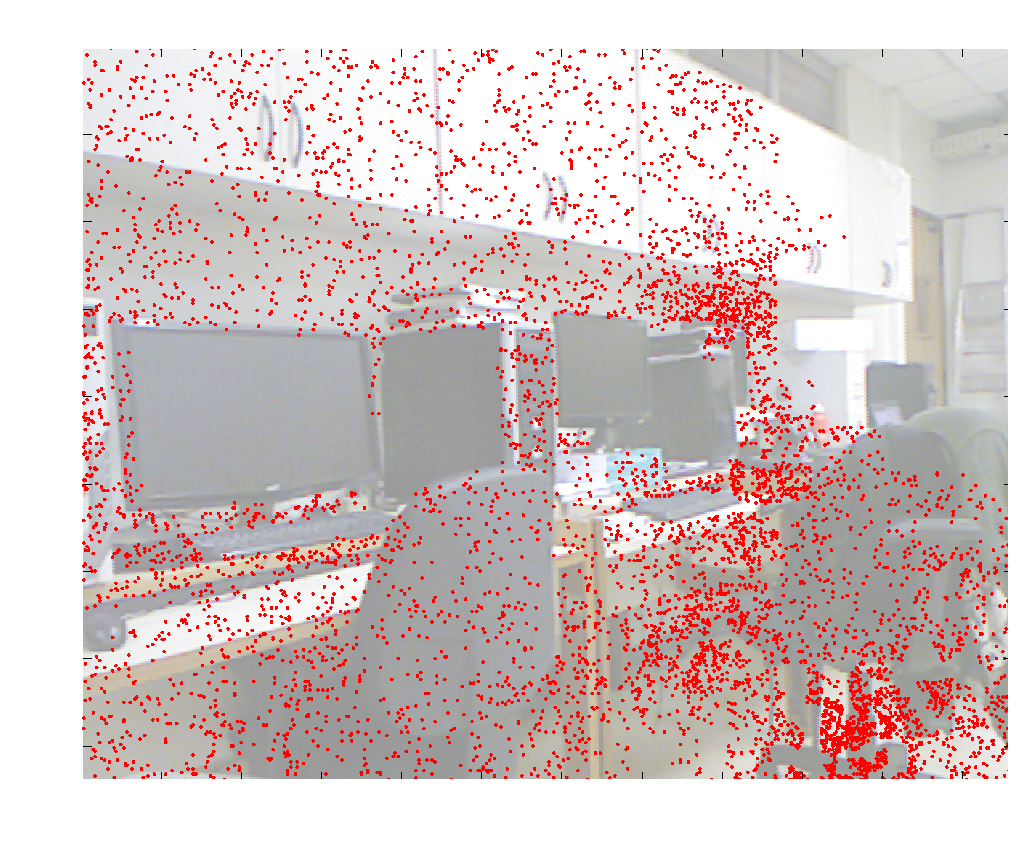
\includegraphics[width=.3\textwidth]{m_csamples.pdf}} \quad
\subfloat[Triangulation $T$]{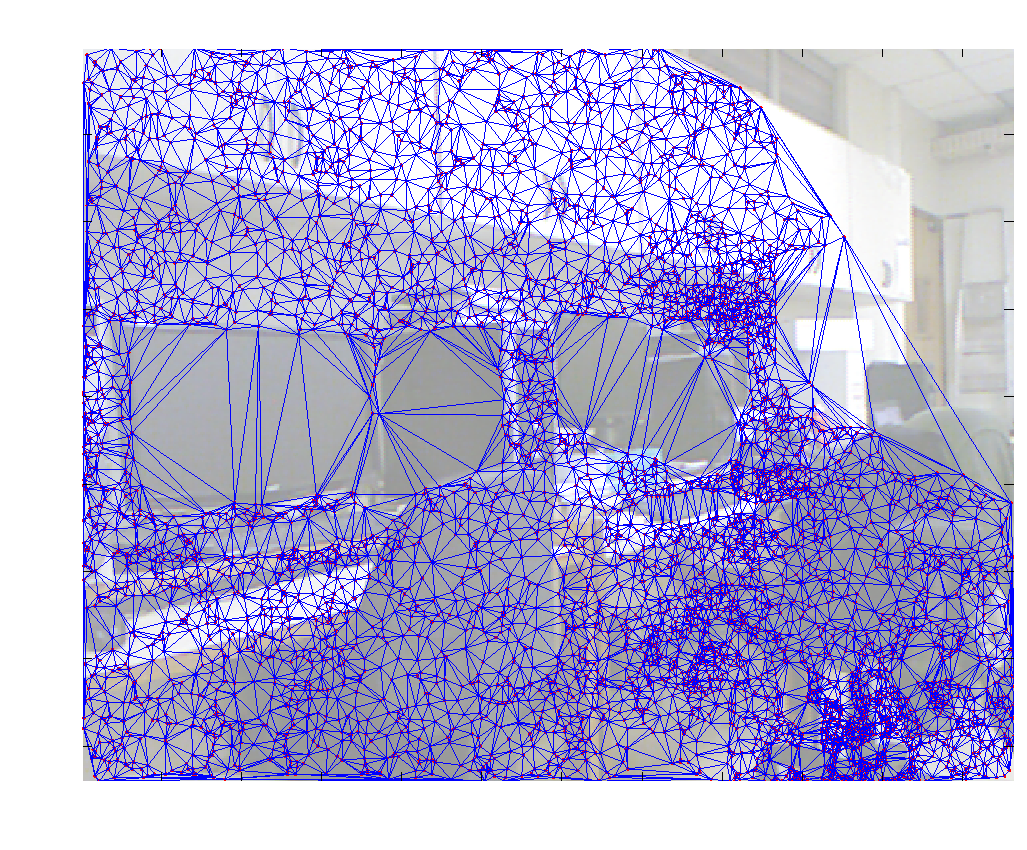
\includegraphics[width=.3\textwidth]{m_ctr.pdf}} \\
\caption{An example of the Triangulation Process. The idea is to start
with a input depth image $D$ and output a triangulation $T$ which has a
topology which is adaptive to the frequency content of the scene.}
\label{fig:O_CT}
\end{figure}

\subsubsection{Frequency Response Image}

The objective of this step is to use image processing techniques to
quickly give an estimate of the frequency content in the depth image
$D$. The end product will be an image $F$ which is the same size as $D$
and will have high values in regions with high change. In order to accomplish
this we will use a sequence of image convolutions. Equation \ref{eqn:HF}
gives the mechanics of the calculation. The Sobel operator $K_S$ is
used to give a response at corners since it is a first order
differential operator. The Laplace operator $K_L$ is used to generate a
response in areas of curvature since it is a second order differential
operator. The Gaussian operator $K_G$ is used to spread the response to the
neighboring areas.   

\begin{align}
F&=(\ \mid D \ast K_S \mid + \mid D \ast K_L \mid \ ) \ast K_G \label{eqn:HF} \\
 & K_S\text{ -- small Sobel operator}  \notag  \\
 & K_L\text{ -- small Laplace operator} \notag \\ 
 & K_G\text{ -- large Gaussian operator} \notag
\end{align}

\subsubsection{Histogram and Sample for Vertices}

The objective of this section is to use the frequency response image $F$
to create a set of vertices $V$. These vertices will be defined as
locations in $D$. The idea is to have a denser number of vertices in
regions of $D$ which have a high frequency content. In order to
accomplish this, we first define regions of similar frequency content by histogramming $F$. An
example of this histogramming can be seen in Figure \ref{fig:O_CT}d.
Next we will probabilistically sample $F$ to define a
set of vertices $V$. The probability of each pixel being sampled is 
given by Equation \ref{eqn:vpr}. The probability is calculated by the
product of two different weights: $W_F$ is based on the region of $F$
where the measurement comes from and $W_A$ is the proportional area of
that region. The result of sampling for vertices can be seen in Figure
\ref{fig:O_CT}e. In addition, because the probability of picking each
pixel as a vertex can be calculated independently the process is
parallelizable.   

\begin{align}
p(u,v) = W_F(u,v)*W_A(u,v)
\label{eqn:vpr}
\end{align}

\subsubsection{Determine Connectivity}

Here we will use 2D Delaunay triangulation to define a connectivity
between the set of vertices $V$ found in the previous step. We are able
to define the connectivity in $\scriptstyle{\mathbb{R}}^2$ space because
the topology is conserved as we project the elements into
$\scriptstyle{\mathbb{R}}^3$.


\subsection{Classification Process}

The goal of the classification process is to use the difference between
the actual depth image and the expected to classify regions of the depth
image by the effect they will have on the model. In order to generate an
expected depth image $E$ we will use the existing mesh map $M$ and the
known pose of the sensor $P$ to create an artificial depth map of the of
what we expect the sensor to see $E$. We can then use image differencing
and binary blob detection to segment regions of the depth map $D$.  

\begin{figure}[h]
  \centering
    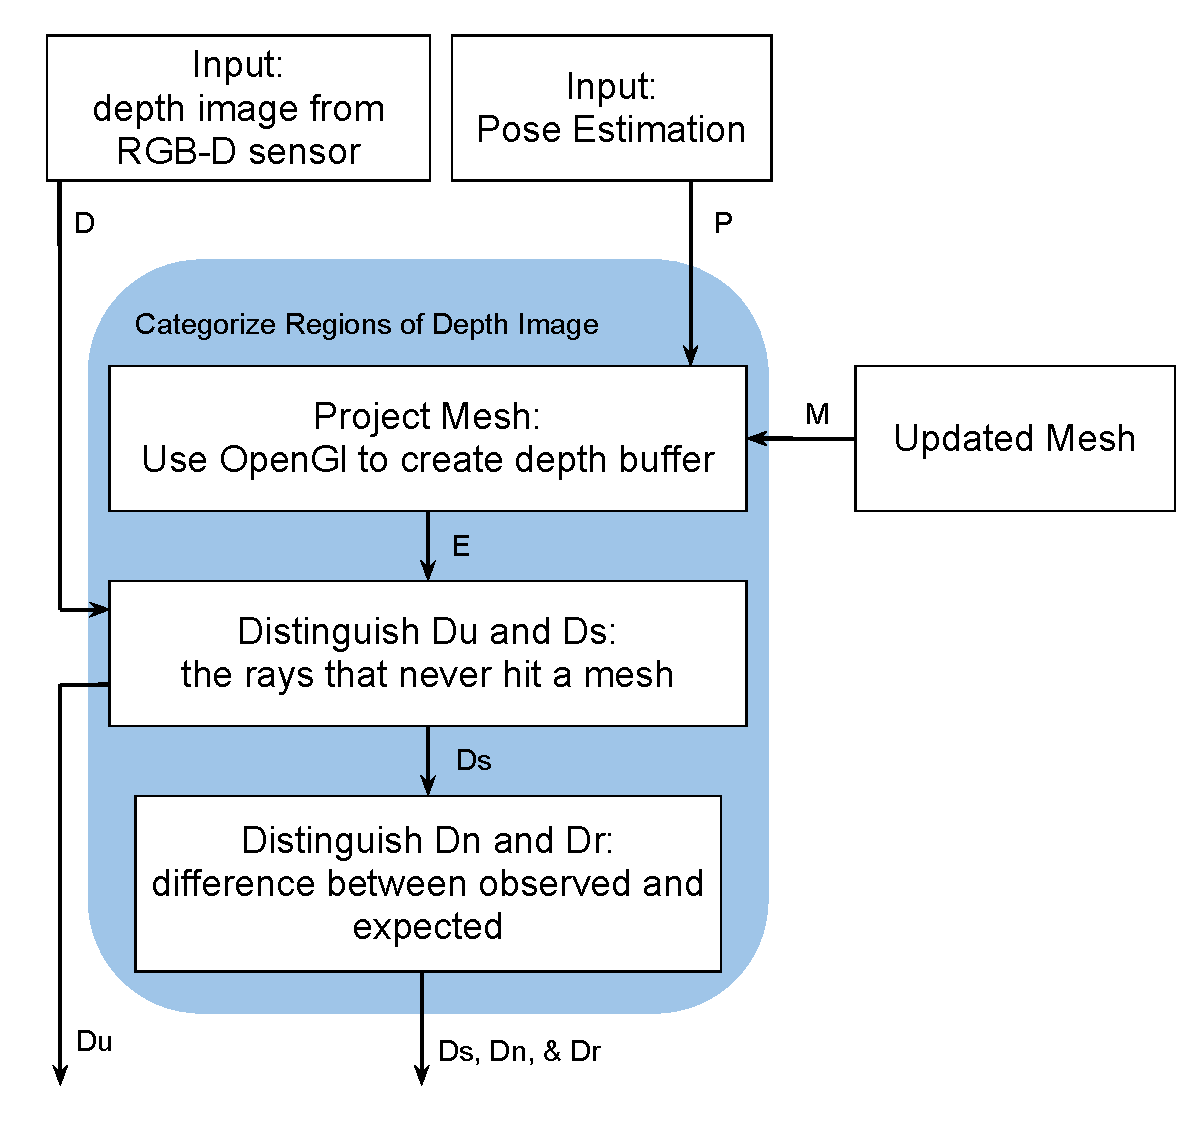
\includegraphics[height=0.5\textwidth]{SD_CM.pdf}
  \caption{Flow Diagram of Categorize Measurements Process}
  \label{fig:SD_CM}
\end{figure}

\subsubsection{Generate Expected Depth Image $E$}

We will use an existing graphics code library named OpenGL to generate
an expected depth image $E$.  A similar approach was used by Fallon et
al. in  \cite{Fallon2012}.  Figure \ref{fig:proj} is a figure from
Fallon's paper which gives a clear idea of the proposed method. The
procedure will be to give the existing mesh model $M$ and the current
pose $P$ to OpenGL and render a depth buffer. It is possible to define the
intrinsic parameters of the sensor to match the actual sensor. Figure
\ref{fig:proj}a and \ref{fig:proj}b give an example of this process.
Figure \ref{fig:proj}b represents the output of this step being the
expected depth image $E$.   

\begin{figure}[h]
  \centering
    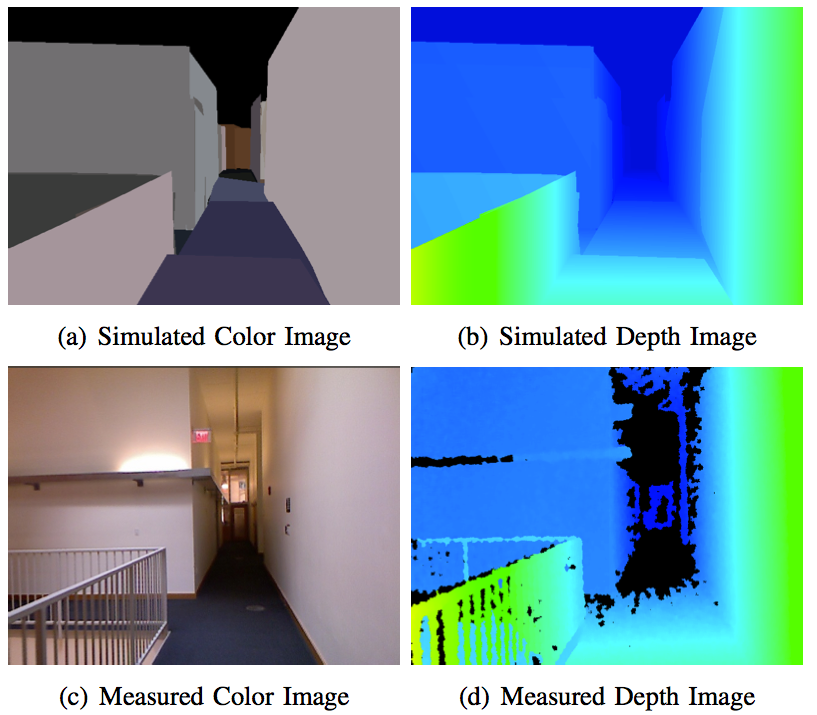
\includegraphics[height=0.7\textwidth]{m_proj.png}
  \caption{Work from \cite{Fallon2012} which generates an expected depth image $E$
in the same way as the proposed method.}
  \label{fig:proj}
\end{figure}

\subsubsection{Find Unknown Parts of the Scene}

The objective of this step is to determine regions of the depth image
$D$ which correspond to areas of the environment which have never been
seen before. This will be accomplished by finding regions of $E$ which
have no measurement. This occurs when the ray traced through the pixel
never hits a mesh element. Regions which are unseen will be designated
as $D_U$ and the rest will be designated as $D_S$. 

\subsubsection{Find New and Removed Objects}

The objective of this step is determine if measurements from the known
region of the environment $D_S$ correspond to new $D_N$ or removed $D_R$
objects in the scene. If they do not belong to $D_N$ or $D_R$ then they
support an existing surface in the mesh map. Essentially they belong to
a supporting region $D_S$ until proven otherwise. In order to prove
otherwise we will use image differencing between the expected $E$ and
the seen parts of the environment $D_S$. We will threshold the
differenced image with $-\epsilon$ and $+\epsilon$ to make two distinct
binary images. Blob analysis will then be run on this image to determine
$D_N$ and $D_R$.  

\subsection{Update Mesh}

This is the last and most important step of the proposed method. Here
we will combine the triangulation $T$ found in the Triangulation Process
and the regions $D_N$, $D_S$, $D_R$, and $D_N$ found from the
Classification Process to efficiently update the existing mesh map $M$. 

\subsubsection{Add or Remove Mesh Elements}

If the measurements in $D$ correspond to new objects $D_S$ or to unseen
parts of the environment $D_N$, new mesh elements will need to be added.
The new elements will come from the triangulation defined in $T$. In
order to successfully merge the new elements with the existing mesh $M$
the bordering vertices of the region will need to be found and stitched.
It is proposed that this merging operation can be done in $D$. 

If the measurements in $D$ correspond to removed objects $D_R$, then the
elements are removed from $M$. This is done by marking the vertices
within the $D_R$ region and deleting them and their connections.  

\subsubsection{Adapt Existing Mesh}

Regions of the depth map which support an existing surface of the mesh
model will be used to adapt the mesh in order to better approximate the
real world. The idea of this process can be seen in Figure
\ref{fig:AM}. In this figure the real world is represented by the blue
surface in Figure \ref{fig:AM}a. The red dots represent the measurements
from $D$. The mesh $M$ is represented by the green surface. In the
figure we see a single vertex being adjusted. In Figure \ref{fig:AM}b a
set of planes are defined at the surrounding vertices and through the
measurements which correspond to this particular vertex. This
neighborhood of measurements will be found by defining a neighborhood in
$D$. In Figure \ref{fig:AM}c the vertex is adjusted. This adjustment
will be done by applying the Quadratic Error Measurement (QEM). The QEM
will adjust the vertex to minimize the distance between all planes which
were found in Figure \ref{fig:AM}b.    

\begin{figure}[h]
\centering
\subfloat[Vertex with neighboring measurements]{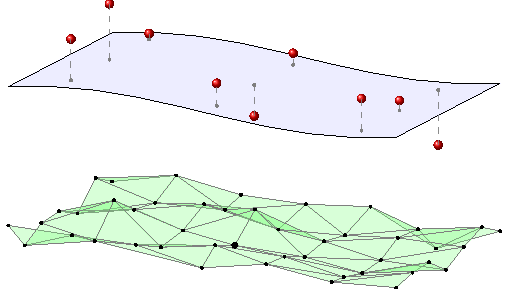
\includegraphics[width=.3\textwidth]{AM1.pdf}} \quad
\subfloat[Fitting a plane at neighboring vertices and through
neighborhood of measurements]{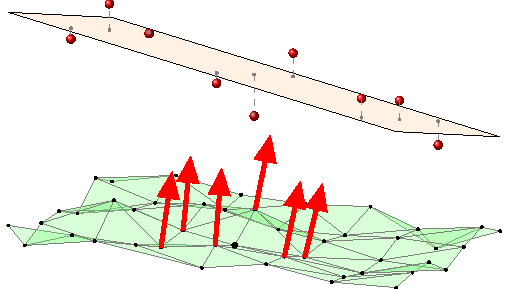
\includegraphics[width=.3\textwidth]{AM2.pdf}} \quad
\subfloat[Movement of vertex based on QEM]{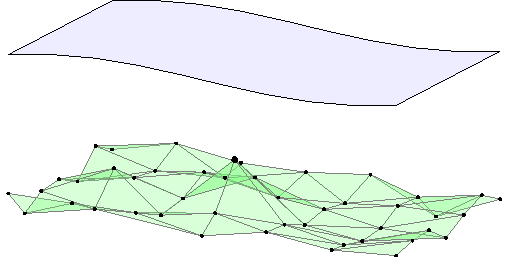
\includegraphics[width=.3\textwidth]{AM3.pdf}} \\
\caption{This shows the process of adapting a single vertex with new
measurements. }
\label{fig:AM}
\end{figure}

\section{Validation}
\label{ch:validation}

In order to evaluate and quantify the effectiveness of the proposed mapping
methodology, a series of experiments will be run in simulation.  The reason
for validating through simulation is that we will have control of all
aspects of the experiment. In addition, we will have a known position of
the sensor in a known environment. This will allow us quantitatively measure
our error. Figure \ref{fig:Sim} gives an idea of how the simulation will be
accomplished. We will use a 3D modeling software named blender to create the
environment and save it to a .ply file. Then, we will use OpenGl to open
the .ply file and simulate readings from an RGB-D sensor. Finally, we will
port these measurements to Matlab where the proposed mapping algorithm will
be developed and tested. 

\begin{figure}[h]
\centering
\subfloat[Define geometry in Blender]{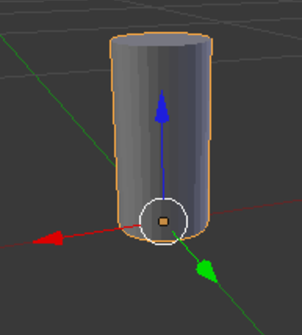
\includegraphics[width=.3\textwidth]{Sim1.pdf}} \quad
\subfloat[Render depth map in OpenGl]{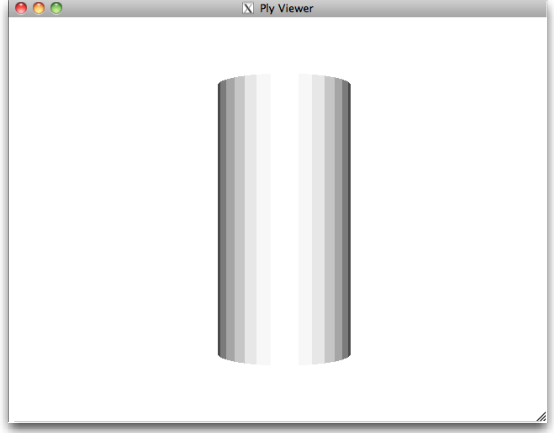
\includegraphics[width=.3\textwidth]{Sim2.pdf}} \quad
\subfloat[Export depth image to Matlab]{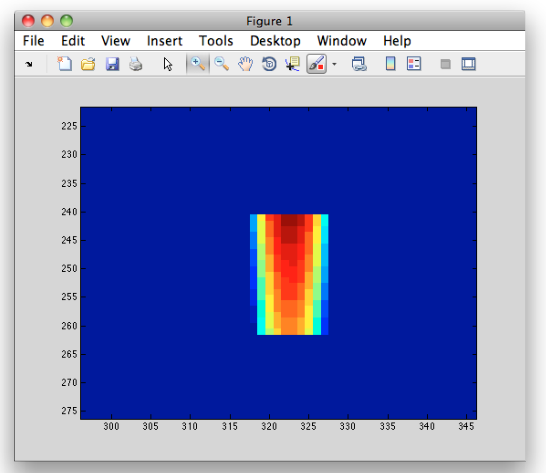
\includegraphics[width=.3\textwidth]{Sim3.pdf}} \\
\caption{The steps of the simulation pipeline. The pipeline will allow
us to simulate a RGB-D sensor viewing a known environment with a known
pose.}
\label{fig:Sim}
\end{figure}

With this simulation pipeline we can design a set of experiments which will
sequentially test the abilities of the proposed mapping system. The idea
will be to start with the easiest tests first in order make sure the system
can map the environment under the most ideal conditions. Then, each
subsequent experiment will aim to test a particular part of the system. By
testing in this sequential manner we will be able to isolate and
troubleshoot problematic parts of the system. Consequently, we will gain
greater insight on the behavior of the system as a whole and the final
system will be robust. The last experiment will test the robustness of the
system with real world data. The following lists the proposed experiments
and briefly describes the intention behind each experiment. For discussion
purposes we can envision an environment which is made of a table and a can
on the table. 

\begin{enumerate}
\item Static scene; static object; static sensor \\
Here we will test the system under the most ideal conditions. We want to
see that the system will categorize all measurements as $D_S$ after the
initial mesh is created. We will also test the ability of the system to
adapt the current mesh over time.  
\item Static scene; static object; dynamic sensor \\
Here the sensor will move in the environment. For example, we can have it
pan across the table by 1 meter. We want the system to recognize
measurements which are from unseen parts of the environment and categorize
them as $D_U$. Also, we want new elements to be added in unknown regions
using the triangulation $T$ from the Triangulation Process.  
\item Dynamic scene; static object; static sensor \\
This experiment will test the ability of the system to detect new and
removed objects. We will do this by spontaneously adding and removing a
second object in the scene such as another cup on top of the table. We will
be looking for the system to successfully categorize the measurements as
either $D_N$ or $D_R$. We will then test the ability of the system to
quickly remove or add the corresponding mesh elements from the current
mesh. 
\item Dynamic scene; dynamic object; static sensor \\
This experiment will also test the ability of the system to react to new or
removed object, however the object will be moved into place over time. This
will be a much more thorough testing of the Categorization Process and the
ability to quickly add and remove elements. 
\item Dynamic scene; dynamic object; dynamic sensor \\
This experiment will test the entirety of the system in simulation. We can
have the sensor circle the table while new elements are being added and
removed. 
\item Real world data \\ 
This test will show the ability of the system to work with real world data
from a RGB-D sensor. We will make use of an open source data set which is
complete with pose information. 
\end{enumerate}

\section{Tasks}
\label{ch:tasks}

There are six major phases which will need to be completed for this
research. The following sections will list the steps which must be
completed for each phase. 

\subsection{Simulation Pipeline}

\begin{itemize}
\item Model all needed environments and object in Blender.
\item Simulate a RGB-D sensor viewing the environments using OpenGL.
\item Read in the simulated sensor output to Matlab.   
\end{itemize}

\subsection{Triangulation Process}

\begin{itemize}
\item Calculate frequency response image $F$
\item Sample $F$ to obtain vertices $V$
\item Triangulate vertices to obtain $T$
\end{itemize}

\subsection{Classification Process}

\begin{itemize}
\item Generate expected $E$ from current mesh $M$
\item Image differencing and blob analysis
\end{itemize}

\subsection{Map Update}

\begin{itemize}
\item Adaptation procedure
\item Add/remove elements
\end{itemize}

\subsection{Experiments}

Run validation experiments 1-6 as discussed in the Validation section. 

\section{Gantt Chart}
\label{ch:ganttchart}

In order to complete this work it will be necessary plan the completion of
the major tasks which were listed in the Tasks section. Figure \ref{fig:GC}
shows a Gantt Chart with the deadlines for each of the 5 major tasks and
also shows the time needed for writing the Thesis. The Simulation Pipeline
will be created first in order to have a database which will be used in
code development of the other processes. It is important to note that some
prior code development has been started and is represented by the gray
portion of the task bars in Figure \ref{fig:GC}. I plan to defend my thesis
April 15th.    

\begin{figure}[h]
\begin{center}
\begin{ganttchart}[y unit title=0.4cm,
y unit chart=0.5cm,
vgrid,hgrid, 
title label anchor/.style={below=-1.6ex},
title left shift=.05,
title right shift=-.05,
title height=1,
bar/.style={fill=gray!50},
incomplete/.style={fill=white},
progress label text={},
bar height=0.7,
group right shift=0,
group top shift=.6,
group height=.3,
group peaks={}{}{.2}]{28}
%labels
\gantttitle{February}{4}
\gantttitle{March}{16}
\gantttitle{April}{8} \\
\gantttitle{Week 1}{4} 
\gantttitle{Week 2}{4} 
\gantttitle{Week 3}{4} 
\gantttitle{Week 4}{4} 
\gantttitle{Week 5}{4} 
\gantttitle{Week 6}{4} 
\gantttitle{Week 7}{4} \\ 
%tasks
\ganttbar[progress=40]{Simulation Pipeline}{1}{4} \\
\ganttbar[progress=75]{Triangulation Process}{4}{7} \\
\ganttbar[progress=0]{Classification Process}{7}{12} \\
\ganttbar[progress=0]{Map Update}{12}{16} \\
\ganttbar[progress=10]{Validation}{16}{20} \\
\ganttbar[progress=0]{Write Thesis}{20}{28} \\
\end{ganttchart}
\end{center}
\caption{Gantt Chart}
\label{fig:GC}
\end{figure}

\end{document}


